\documentclass[12pt]{article}
\usepackage[utf8]{inputenc}
\usepackage{amsmath, amssymb, amsthm}
\usepackage{graphicx, float}
\graphicspath{{Fritzing/}, {SchemiDrawio/}, {Servizi/}, {Loghi/}}
\usepackage[a4paper,top=2cm,bottom=2cm,left=2.5cm,right=2.5cm,heightrounded]{geometry}
\usepackage{parskip}
\usepackage{enumitem}
\setlist[itemize]{label= -}
\usepackage[italian]{babel}
\usepackage{hyperref}
\hypersetup{
    pdfborder={0 0 0}
}

\title{ \Huge{\textbf{sMister}}\\
        \normalsize{Sistema di smistamento pacchi automatico}
        }

\author{Massarutto Thomas - 158502\\
        Scaini Luca - 666666
        }
\date{\today}

\begin{document}
\pagenumbering{gobble}
\maketitle

\begin{figure}[H]
    \centering
    
\includegraphics[width=0.5\linewidth]{Uniud.png}
    \label{logo uniud}
\end{figure}

\section*{GitHub}Link repository GitHub: \href{https://github.com/Scaini99/Progetto_IOT}{\textbf{sMister}}

\section*{Autori}
Massarutto Thomas: \href{mailto:158502@spes.uniud.it}{158502@spes.uniud.it}

Luca Scaini: \href{mailto:666666@spes.uniud.it}{666666@spes.uniud.it}


\newpage
\pagenumbering{Roman}
\tableofcontents

\newpage
\pagenumbering{arabic}
\section{Idea}

L'idea di sMister nasce dalla crescente necessità da parte delle aziende di sistemi automatizzati che rendano più veloce ed efficiente lo smistamento dei pacchi. Questo sistema permette ad un centro logistico di ottimizzare il processo di consegna calcolando i percorsi ottimali per i corrieri e gestendo il flusso dei pacchi dal magazzino fino al veicolo di consegna.

Obiettivi del progetto

\begin{itemize}
    \item Ottimizzare i percorsi dei corrieri per migliorare l'efficienza delle consegne
    \item Ridurre al minimo l'intervento umano nella gestione dei pacchi
    \item Realizzare un sistema facilmente replicabile e scalabile
    \item Limitare la dipendenza da servizi di terze parti
\end{itemize}

\section{Tecnologie}

\subsection{Hardware}
Per quanto riguarda la piattaforma hardware, si è scelto di utilizzare un Raspberry Pi 5 ovvero un single board computer sufficientemente prestante da supportare un sistema operativo e dotato di pin GPIO utili per il collegamento di componenti esterni. 

La lettura dei codici identificativi dei pacchi viene eseguita da una telecamera USB, mentre l'hardware per lo smistamento fisico dei pacchi è stato collegato tramite l'interfaccia GPIO.

La componentistica utilizzata è:

\begin{itemize}
    \item motore stepper: attiva il nastro trasportatore 
    \item sensore ad ultrasuoni SR04: rileva il passaggio del pacco davanti alla postazione di smistamento relativa alla baia di carico
    \item motore stepper: attiva il diverter che devia il pacco verso la zona del veicolo per la consegna
\end{itemize}

Per motivi di costo si è deciso di non utilizzare telecamere davanti ad ogni postazione di smistamento e di utilizzare dei sensori ad ultrasuoni che sono più economici e facili da reperire. Sensori laser sarebbero stati equivalenti, tuttavia non erano disponibili al momento dell'assemblaggio.

\begin{figure}[H]
    \centering
    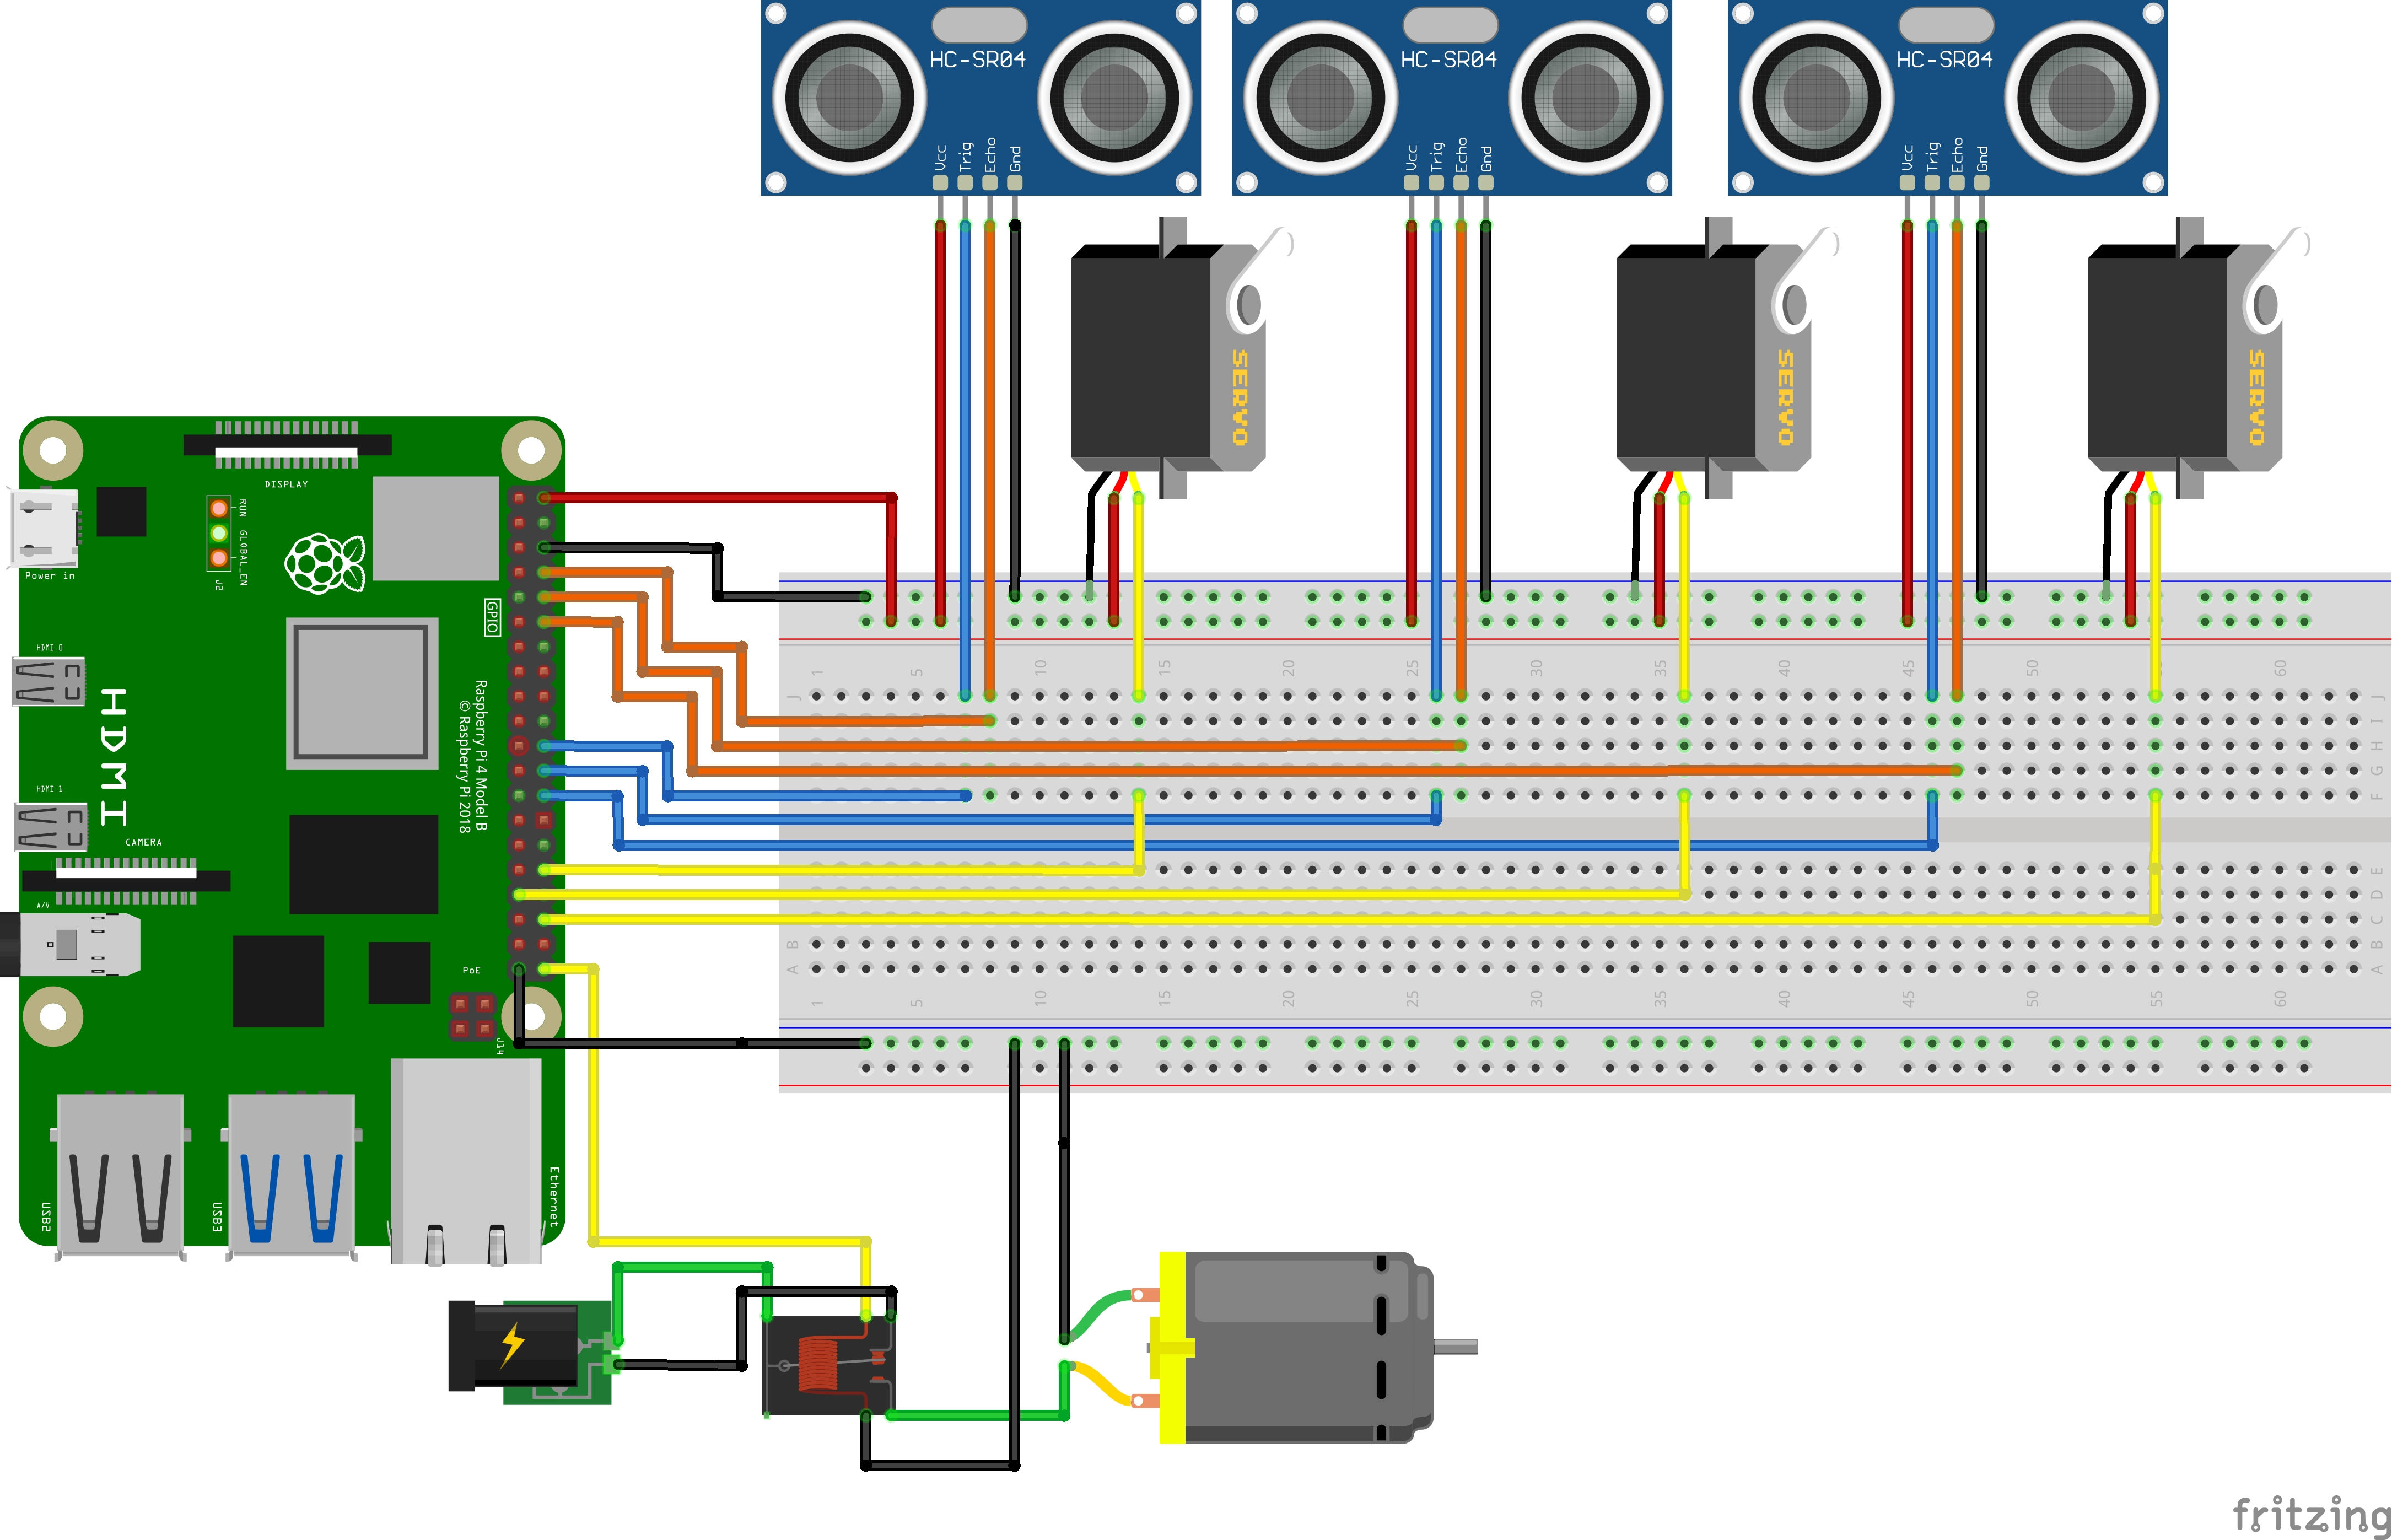
\includegraphics[width=0.5\linewidth]{smister_bb.jpg}
    \caption{Collegamenti Hardware}
    \label{immagine1}
\end{figure}

\subsection{Software}
Il core del progetto è stato sviluppato in Python. Questo linguaggio è stato scelto per via della sua facilità di prototipazione e dell'ampia disponibilità di librerie.

Per garantire un approccio modulare e flessibile sono state sviluppate due librerie custom: \texttt{vroom\_utils} e \texttt{conveyoryeeter}.

Vroom\_utils è la libreria che astrae la comunicazione con i servizi di routing. Funge da interfaccia per le componenti principali di Vroom, come \texttt{job} e \texttt{vehicle}, e viene usata per generare le richieste con metodi ad alto livello che rendono il codice principale più leggibile.

Conveyoryeeter è la libreria che si occupa di astrarre a livello software i componenti hardware del sistema di smistamento. Le periferiche hardware come i sensori ad ultrasuoni, il motore del nastro trasportatore e i motori per i diverter sono gestiti tutti da questa libreria. Ogni stazione è composta da un sensore di rilevazione del pacco e da un diverter. Grazie ad uno stato stato interno il sistema è in grado di capire, al passaggio di un pacco, se questo deve essere deviato verso la relativa baia di carico o se deve essere lasciato passare.

\begin{figure}[H]
    \centering
    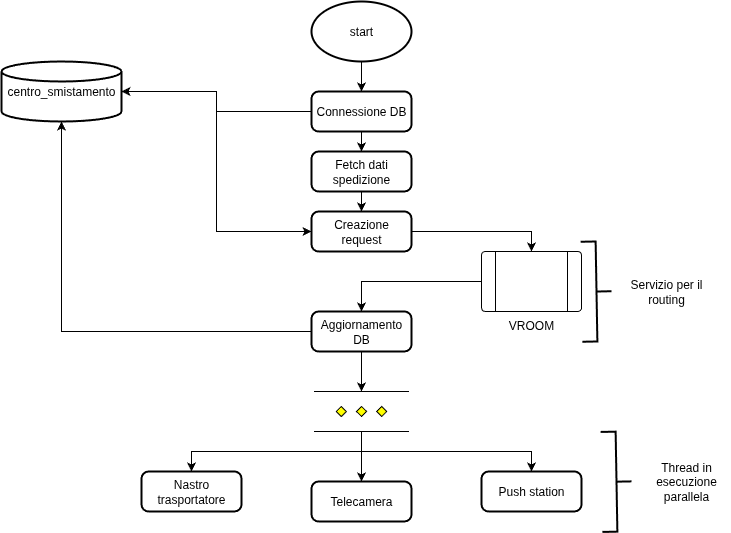
\includegraphics[width=0.5\linewidth]{sMister-Processo_generale.drawio.png}
    \caption{Grafico di funzionamento di tutto}
    \label{imamagine2}
\end{figure}

\subsection{Servizi}

Parte fondamentale del progetto sono i servizi Docker che permettono al sistema di essere facilmente configurabile e integrabile in vari ambienti grazie a vari servizi Docker installati in locale. Sono stati usati i seguenti servizi:

\begin{itemize}
    \item Portainer: interfaccia grafica web che permette l'installazione di container in maniera semplificata
    \item Postgres: il database che contiene le informazioni relative ai pacchi
    \item Adminer: programma che serve per gestire da un interfaccia grafica Postgres
    \item VROOM: servizio che fornisce un sistema di routing ottimale
    \item OSRM: motore open source per il calcolo di percorsi stradali
\end{itemize}

I servizi sono stati organizzati in stack dedicati, in modo da raggruppare componenti funzionalmente simili.

\section{Funzionamento}
sMister interroga il database per ottenere l'elenco delle consegne previste e riceve come risposta gli indirizzi dei colli associati. Queste informazioni sono trasformate in jobs, ovvero lavori di consegna da effettuare e, in base alla flotta di veicoli per le consegne disponibili, delega a VROOM il calcolo dei percorsi ottimali per ogni veicolo. 

Una volta calcolato ciò, il sistema deve riconoscere l'id del pacco su un nastro trasportatore per indirizzarlo verso la baia di carico corretta: questo viene fatto tramite un codice a barre che identifica unicamente ogni pacco. Lungo la linea alcuni attuatori si occupano di consegnare alla zona di carico giusta ogni pacco.

\subsection{Fasi}
Il sistema funziona in varie fasi separate e sequenziali.

\subsubsection{Requisiti}

I requisiti perché il sistema possa funzionare sono quelli di avere una connessione ad un database con le informazioni riguardanti i pacchi presenti in magazzino. È necessario che ogni pacco abbia un codice univoco, un indirizzo di spedizione e uno stato che indica se il pacco sia ancora da consegnare o meno (ritiri in sede, consegne mancate, ...). 

\subsubsection{Fase 1}

Una volta avvenuta la connessione al database, \emph{sMister} lo interroga richiedendo i pacchi con il flag specifico per la consegna in data odierna. 

\end{document}